To better visualize the context of this thesis work, it is essential to introduce the main system paradigms that today guide the various security certification frameworks.

\section{Cloud Computing Paradigm}
The National Institute of Standards and Technology (NIST) defined the Cloud computing paradigm as follows: “Cloud computing is a model for enabling ubiquitous, convenient, on-demand network access to a shared pool of configurable computing resources (e.g., networks, servers, storage, applications, and services) that can be rapidly provisioned and released with minimal management effort or service provider interaction \cite{mell2011nist}."

The most commonly used deployment model for Cloud computing is the public Cloud, which allows users to access its resources through the Internet and is generally subject to monetization from provider companies.
Another commonly used deployment model is the private Cloud, usually found in single organizations for a more secure digital environment.
The other two models are Hybrid Cloud and Community Cloud, where the former is a mixture of public and private Cloud that overcomes some of the limitations of each, and the latter is an expansion from a private cloud, allowing multiple organizations to access its resources \cite{atlam2017integration}.

The essential services that Cloud computing offers include infrastructure as a service (IAAS), platform as a service (PAAS) and software as a service (SAAS), each of whom allows a different calibre of resources' control between the user and the provider \cite{khan2019edge}.

%%%%%%%%%%%%%%%%%%%%%%%%%%%%%%%%%%%%%%%%%%%%%%%%%%%%%%%%%%%%%%%%%%%%%%%%%%%%%%

\subsection{IoT In Cloud Environments}
Given the general flexibility, dynamicity and resource availability of Cloud computing, it has been the first adopted solution for IoT (Internet of Things) systems implementations.
The IoT label defines the network created around small smart devices interconnected through the Internet. To be classified as an IoT device, a piece of hardware has to be embedded with electronics, software, and connectivity in a way that enables it to communicate with other devices and exchange data that can be directly gathered from the device itself thanks to specific embedded sensors or from other connected devices.
The range of possible objects that today are intended as Smart IoT devices is vast; it comprehends instruments, vehicles, buildings, all sorts of sensor-enabled devices \cite{gokhale2018introduction}, industrial machines, and small objects like clothing, packages, parts, materials and much more. All these objects are active participants in the network and thus can be monitored, tracked and counted.
Cloud computing and IoT are built with complementary ideas; on the one hand, the Cloud is ubiquitous, secure, flexible and equipped with such a broad resource capability that it is often referred to as infinite. However, on the other hand, IoT devices are distributed and capable of generating immense moles of data that need a powerful computing element to analyze and process them.
Cloud computing simplifies the IoT data flow significantly and helps overcome many devices' limitations such as security, privacy, performance, and reliability. The main benefits of IoT integration in Cloud environments are widely discussed in \cite{atlam2017integration}.

As mentioned above, IoT devices generate a significant constant flow of data that for sure cannot be handled by the small devices themselves, but that is also becoming an issue for the Cloud infrastructures since IoT systems grow bigger and bigger every year, with more sensors and more communicating units [need source].
The biggest challenge in the IoT field is managing the massive quantity of data generated, and even the Cloud solutions are challenged by the large scale, heterogeneity and high latency issues. One rapidly increasing solution in popularity consists of using a decentralized computing model known as Fog Computing \cite{iorga2018fog}.

%%%%%%%%%%%%%%%%%%%%%%%%%%%%%%%%%%%%%%%%%%%%%%%%%%%%%%%%%%%%%%%%%%%%%%%%%%%%%%

\section{Edge Computing Paradigm}
Edge computing directs computational data, applications, and services away from Cloud servers to the edge of a network. The content providers and application developers can use the Edge computing systems by offering the users services closer to them. Edge computing is characterized in terms of high bandwidth, ultra-low latency, and real-time access to the network information that can be used by several applications \cite{khan2019edge}.

Edge or Fog computing is the latest and most promising researched solution to the recent trends of distributing the computation closer to the data sources. The goal is to provide low latency, high capacity and network efficient computation to IoT systems bringing multiple small Cloud nodes (Fog nodes) between the Cloud and the IoT devices at the "edge" of the network. As for many concepts, the definitions are numerous \cite{sahni2018data} but Yi et al. stated the following as a possible definition: "Fog Computing is a geographically distributed computing architecture with a resource pool which consists of one or more ubiquitously connected heterogeneous devices (including edge devices) at the edge of the network and not exclusively seamlessly backed by Cloud services, to collaboratively provide elastic computation, storage and communication (and many other new services and tasks) in isolated environments to a large scale of clients in proximity" \cite{yi2015fog}.
Practically Fog computing represents an extension of Cloud computing that offers multiple benefits to the latter:

\begin{itemize}
    \item Location awareness and low latency
    \item Geographical distribution
    \item Scalability
    \item Support for mobility
    \item Real-time interactions
    \item Heterogeneity
    \item Interoperability
    \item Support for online analytics and interplay with the Cloud
\end{itemize}


\subsection{Edge And Cloud Relationship}
Edge computing is considered an extension of Cloud computing and not a standalone computing paradigm; it still relies on the Cloud at the top level of its scheme, but it drastically reduces the load over the Cloud infrastructures while maintaining all of the Cloud's provided services like data computing, storage and applications. The main difference between the two is the location of the servers; with the Cloud alone, latency dependant applications may encounter latency and jitter issues due to the distance between the user device and the server. On the other hand, Edge computing enables location-aware and mobile applications with full support, while Cloud applications need to find other workarounds. The longer path to the server can also be a weak point for security attacks on the Cloud. Another difference is the target audience: Cloud computing is a global solution, Edge computing is limited. Lastly, the single Edge node hardware is designed to be horizontally scalable through distribution, while Cloud computing is generally more vertically scalable \cite{khan2019edge}.


Today, an ever-rising number of applications must use software that satisfies strict reliability, availability and integrity requirements, especially when dealing with critical safety systems; hence, multiple assurance and verification techniques have been introduced, such as certification schemes, testing, service level agreements, audit/compliance and monitoring frameworks \cite{ardagna2015security}. 


\section{Security Certifications}
Security certifications are granted by independent (from the system supplier and acquirer) third parties whose goal is to verify the system's quality completely and objectively. Certifications allow more confidence in the product over the competition and legislative compliance when talking about quality, functionality and security \cite{heck2010software}.

The certification schemes' main focus is to prove that the selected software system or service would have some non-functional properties and behave as expected. 
Over the years, there have been proposed two main types of certification approaches: i) static, such as the ones proposed by \cite{anisetti2013test}\cite{CSATrustSTAR} ii) continuous and incremental, such as Common Criteria \cite{anisetti2017semi}\cite{infrastructure2002common}. 

A generic software certification process requires two types of input: i) The software artefact that needs to be certified and ii) one or more Conformance Properties of the artefact. The properties usually fall into one of the following categories:

\begin{itemize}
    \item Consistency
    \item Functional
    \item Behavioural
    \item Quality
    \item Compliance 
\end{itemize}

Although in the most recent years, the NIST proposed to definitely classify the systems' properties under just the Confidentiality, Integrity and Availability categories, more about this in the [properties] chapter. 

Moreover, the properties can be generic or dedicated to the specific artefact and need to be appropriate to the application's domain; this is established in a Conformance Analysis process \cite{anisetti2017semi}.


\subsection{Certification Schemes History}
It is quite difficult to retrace the full history of software security certification schemes due to the vastity of the software products' types and the fact that many countries started developing their certification schemes when such products needed some form of assurance. For these reasons, software products requiring security properties resulted in having a rather steep way toward international distribution. Therefore, the first approaches started dealing with the main pillars of certification schemes, such as properties, models and evidence collection (Fig. \ref{Fig:OldProcess}). Starting from the history of the most known scheme, the Common Criteria, the first attempts at defining a standard approach to such a complex task were made between 1983 and 1993 with the Information Technology Security Evaluation Criteria (ITSEC), the Canadian Trusted Computer Product Evaluation Criteria (CTCPEC) and the Trusted Computer System Evaluation Criteria (TCSEC).
\begin{figure}[htb]
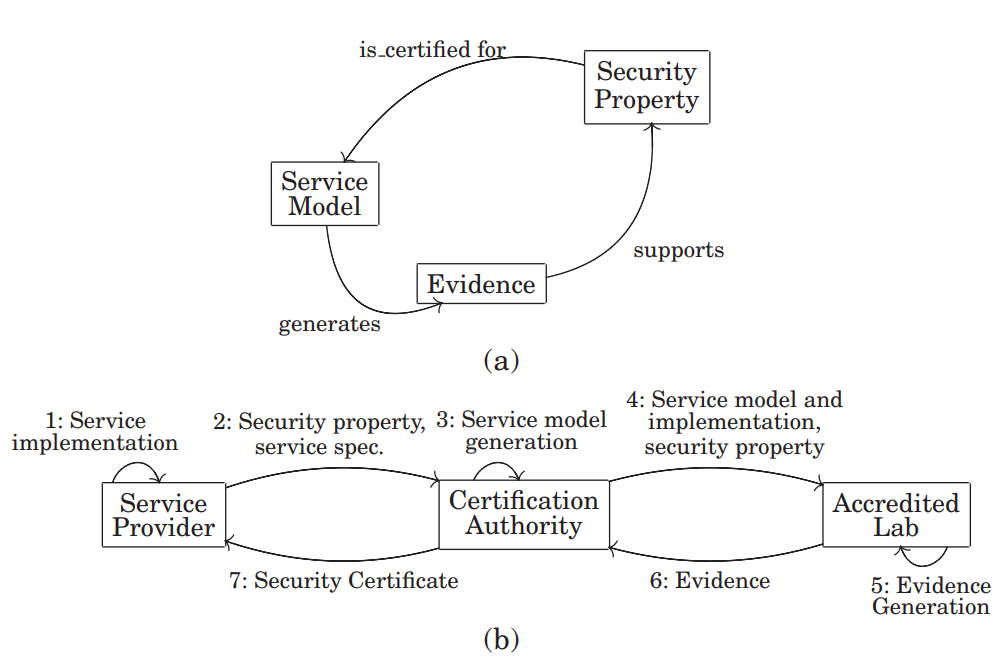
\includegraphics[width=\textwidth]{immagine_web_service.png}
\caption{Conceptual framework (a) and certification process steps (b) \cite{anisetti2013test}}
\label{Fig:OldProcess}
\end{figure}
\subsubsection{ITSEC}
ITSEC is a structured set of criteria with the scope of evaluating security within computer systems and products in the European Union; it was published in 1990 and was developed by France, Germany, Netherlands and UK governments, basing its features on the pre-existing, country-limited frameworks. This set of criteria was designed in the main part to be equally applicable to technical security measures in hardware, software and firmware products \cite{ITSEC}. ITSEC was centred around the Target of Evaluation (ToE) and assurance levels; these concepts made their way through all the versions of today's Common Criteria \cite{infrastructure2002common}.

\subsubsection{TCSEC}
TCSEC, commonly referred to as "The Orange Book" \cite{orangeBook}\cite{orangeBookDeath}, is a standard developed by the United States Government Department of Defense, and its scope was to evaluate and classify computer systems used for processing, storing and retrieving sensitive or classified information. This framework, like many others \cite{infrastructure2002common}\cite{ITSEC}, was developed around the following Evaluation Classes: 
\begin{itemize}
    \item D: Minimal Protection
    \item C1: Discretionary Security Protection
    \item C2: Controlled Access Protection
    \item B1: Labeled Security Protection
    \item B2: Structured Protection
    \item B3: Security Domains
    \item A1: Verified Design
    \item A2: Verified Implementation
\end{itemize}

\subsubsection{CTCPEC}
CTCPEC is a standard developed by the Canadian government with the same goals as ITSEC and TCSEC; in fact, it was a combination of the two. This approach finally led to combining the major standards and criteria into a single set: the Common Criteria \cite{CTCPEC}.

\subsubsection{Common Criteria}
\label{CC}
With these internationally approved standards, software companies finally had the tools to certify their products and sell them worldwide; however, every certification process had to be passed, resulting in a rather tedious and pricey process. Therefore, the Common Criteria (CC) was developed by unifying these pre-existing standards, following the approach of the CTCPEC, to allow companies to evaluate their products against a single set of standards. CC was developed by Canada, France, Germany, Netherlands, UK and USA governments and version 1.0 was issued in 1994; multiple agreements were signed in the following years to avoid useless re-evaluations and allow mutual recognition of CC certificates.
The Common Criteria for Information Technology Security Evaluation (also known as Common Criteria) represents the evolution of continuous and incremental certification schemes, and its latest versions are currently used to evaluate over two thousand major IT systems and applications (e.g. Microsoft Windows OS, McAfee anti-virus, Microsoft SQL Server \cite{CCProducts}).
CC is mainly based on the previous sets of standards' ideas:
\begin{itemize}
    \item Definition of the ToE, which includes the assignment of a Protection Profile, the description of the Security Target and the listing of the Security Functional Requirements.
    \item Definition of the Security Assurance Requirements
    \item Selection of the correct Evaluation Assurance Level
\end{itemize}

More details about the above phases are well described in \cite{infrastructure2002common}.

CC is now an established pillar in the security certification world, especially in the commercial industry, but it is not a perfect solution, especially when applied to highly dynamic systems like Edge and IoT. It is also worth noting that CC certifications are attributed to a specific version of the system under a specific configuration, and any configuration change or software update could mandate a re-certification process. To counter the redundancy of such processes, the CC designers proposed the Assurance Continuity (CCAC) re-evaluation process[], but the need to repeat the certification process is a big limitation. Therefore, the research never stopped; when considering highly dynamic domains such as those implied by the Cloud and Fog computing paradigms, it is important to define new certification schemes that better align with the context. 

\subsection{New Certification Efforts In Cloud Environments}
Cloud service certification has been a highly focused research point in recent years and is now considered a mature assurance feature. Moreover, as identified by M. Anisetti et al. in \cite{anisetti2017semi}: "Compared to traditional service certification, cloud certification is: i) highly dynamic, it is affected by contextual changes at any layer of the cloud stack, ii) multi-layer, it can refer to services at different cloud layers; iii) intrinsically incremental, it requires continuous validity verification and incremental adaptation with the scope to minimize costly re-certification activities, and iv) trustworthy by delegation, it requires advanced trust models based on delegation to support cloud peculiarities". M. Anisetti et al. also proposed a continuous and incremental approach to Cloud service certification, providing a formal description of the audit-related evidence collection. Such an approach is founded on five main pillars: non-functional properties, non-functional mechanisms, Target of Certification (ToC), evidence collection and the life cycle of the certification. The proposed certification process can be simplified with the following steps:

\begin{itemize}
    \item Non-functional properties definition
    \item ToC definition, which includes the description of the non-functional mechanisms offered by the system
    \item Tests definition
    \item Tests execution, which involves evidence collection and analysis
    \item Certificate release
\end{itemize}

This process involves different entities, such as the service provider, the cloud provider, the certification authority and an accredited laboratory; this way, a chain of trust is formed, and the responsibilities are evenly spread between the entities involved. It is also split into an issuing phase, where the process is responsible for all the evaluation activities, and a post-issuing phase, which continuously verifies the certificate's validity against eventual context changes \cite{anisetti2017semi}.

\subsection{New Certification Efforts In Edge Environments}
Certification schemes over Fog/Edge computing nodes are a recent and less mature topic; when dealing with a network composed of countless devices (the Fog nodes), it is fundamental to have a completely automated framework capable of handling the whole certification process for each node. The scheme proposed by Aslam et al. in \cite{aslam2020fonac} addressed the matter with automated and continuous monitoring and auditing of the Fog nodes; nevertheless, this total automation relies entirely on the backend provided by the Cloud infrastructure that acts as an inner CA for its Fog layer, inheriting all its vulnerabilities. The differences between this approach and the ones proposed for the Cloud are the requirements for the certifications. Fog nodes have limited functionalities and need to be quickly admitted to the Fog layer; meanwhile, there is a need to execute much stronger certification activities on the Cloud stack.

\subsection{Current IoT Certification Efforts}
Internet of Things is not a new concept, and so is not the need for dedicated certification schemes; The rapid spread of systems relying on IoT highlighted many limitations of the most known certification schemes.

\subsubsection{Common Criteria}
As described in section \nameref{CC}, CC is the most used on every type of system (Cloud, Edge, IoT) thanks to its Mutual Recognition Agreements (MRA) and to the depth the certification process can reach. However, the industry and the research community have underlined three major limitations that make it hardly applicable in the IoT world \cite{kaluvuri2014quantitative}\cite{keblawi2006applying}:
\begin{enumerate}
    \item It takes too much time and effort, resulting in a slowdown of the system and the risk of overwhelming the single devices with testing requests.
    \item Systems classified with high EALs are attributed to highly complex documentation, making the comparison with other certificates difficult, hence, not complying with the harmonization challenge (more about this in the commercial section).
    \item Managing changes is almost non-existent, even with the CCAC version, limiting the number of updates the manufacturer can issue and drastically reducing system operativity during re-certification.
\end{enumerate}


\subsubsection{ICSA Labs IoT Security Testing Framework}
A newer framework is the one proposed by the ICSA Labs company. The ICSA Labs IoT Security Testing Framework is focused on IoT systems, more specifically, on the security of the single devices participating in an IoT environment. The approach is based on a periodic assessment and update of the certification criteria, and it includes frequent iterative updates, addressing the dynamic environment challenges and the evolving cybersecurity threats inherent to the IoT paradigm. This process is more focused on the iterativity of the assessments and less on the depth of the certification, leaving aspects such as the labelling ignored \cite{ICSAFw}.

CC remains the most used and studied certification scheme, while others like Commercial Product Assurance, Cybersecurity Assurance Program and the Certification de Sécurité de Premier Niveau fall into a commercial and country-specific side.


\subsubsection{Industrial And Commercial Purpose Schemes}
From the commercial and industrial point of view, several challenges have been highlighted in the definition and deployment of an IoT security certification framework; some of these are not part of this thesis' focus but are still relevant for a complete overview of what a certification framework should guarantee at a certain point; furthermore, table \ref{Tab:comparison} shows a quick comparison of the approaches discussed below.
\begin{enumerate}
    \item Standardization: Since the IoT landscape is still fragmented in approaches and standards, it is crucial to start aligning the efforts for a more homogeneous perspective.


    \item Harmonization: while there is the need to align the standards, there is also the need to allow different ones to coexist and be mutually accepted.


    \item Time, complexity and cost: Manual processes, direct testing and complex documentation guidelines of currently available approaches are heavy on resources like time and money, and the need to minimize this weight is crucial for a for-profit company, especially with IoT systems that need frequent re-certifications.


    \item Dynamic environment: IoT systems are often deployed in dynamic environments whose conditions might affect the security level of a device. Moreover, a device should be able to receive an update and change its or the system's configuration without invalidating the certificate completely.


    \item Influence of the context: The context in which an IoT system is deployed is not ignorable; indeed, it determines many of the security features the system will require. Moreover, the context and the system's purpose should be linked to determine the sensitivity of the managed data.


    \item Transparency to the end-user: A company must help the clients understand the positive aspects of the system's certification, especially when different approaches are not directly comparable. For this purpose, it is becoming a common rule to attribute security labels to the certificated devices; such labels should clearly and concisely represent the value of the certification's level. Labels' goal is ultimately to allow users to easily compare different levels of frameworks without knowing the approaches' details.


    \item Support for the certificate lifecycle: cybersecurity certificates carry validity periods that regulate and confirm the authenticity of the involved entities. It is important to ensure that the certification is supported and updated during its lifecycle and that all the certificated properties remain valid during this period.

\end{enumerate}


It should be noted that apart from the AC version of Common Criteria, no other approach considers a lighter process for re-certification processes.

Some available frameworks are adopted more frequently than others; in the following section, the most known and used in the industry will be presented and compared to highlight the major weaknesses that should be considered when developing new certification schemes \cite{surveyIOT}.

\subsubsection{Commercial Product Assurance}
The Commercial Product Assurance (CPA) is a certification scheme developed by the UK Communications-Electronics Security Group (CESG) for national public purposes. CPA allows only security-related patches and updates, and thanks to its "lightweight" design, it drastically reduced the re-certification process length; however, it is not enough. The average re-certification still takes at least six months to complete, reducing the system operativity during this time.

\subsubsection{Cybersecurity Assurance Program}
Cybersecurity Assurance Program (CAP) is a certification methodology developed by the Underwriters Laboratories company (UL) that adheres to their proprietary UL 2900 standards. Unfortunately, being a private and for-profit organization drastically reduces the community's trust in its certificates since they are not provable by third-party experts and do not adhere to the standardization and harmonization challenges.

\subsubsection{Certification de Sécurité de Premier Niveau}
The National Cybersecurity Agency of France developed certification de Sécurité de Premier Niveau (CSPN) in 2008 to verify the products' compliance with their security specifications in a timely manner. Unfortunately, this certification framework is standardized in France but not officially recognized by any other country, making it useless for international products.

%%%%%%%%%%%%%%%%%%%%%%%%%%%%%%%%%%%%%%%%%%%%%%%%%%%%%%%%%%%%%%%%%%%%%%%%%%%%%%%%%%

    


\begin{table}[htb]
    \centering
    \begin{tabular}{ |p{3cm}|p{2.3cm}|p{2cm}|p{2cm}|p{2cm}|p{2cm}|  }
         \hline
         \textbf{Challenges}&\textbf{CC}&\textbf{CPA}&\textbf{CAP}&\textbf{CSPN}&\textbf{ICSA Labs}\\
         \hline
         \textbf{Certification time (months)}* & 4-9 EAL2, 6-12 EAL3, 9-24 EAL4.
         & 6-18 & 6+ & 1-2 & 1-2\\
         \hline
         \textbf{Documentation} & Higher the EAL more complex the documentation & Hard to compare & Hard to compare & Hard to compare & Hard to compare\\
         \hline
         \textbf{Changes management} & Certificate valid only for specific patch and configuration & Any change is manually reviewed and can invalidate the certificate & Any change is manually reviewed and can invalidate the certificate & security patches invalidate the certificate & Any change is manually reviewed and can invalidate the certificate\\
         \hline
         \textbf{Context consideration} & Yes & No & Partially & Yes & Yes \\
         \hline
         \textbf{Monitoring} & Yes & Yes & Yes & No & Yes \\
         \hline
         \textbf{Validity period} & Variable & Variable & 1 Year & 8 Weeks & 1 Year \\
         \hline
         \textbf{Labels completeness} & Only EAL info & None & None & None & None \\
         \hline
         \textbf{Mutual Recognition Agreements (MRA)} & Accepted by numerous countries & UK only & Not standard & France only & Not standard \\
         \hline
         \textbf{Cost (\$)}* & 75-200k EAL2, 110-250k EAL3, 150-350k EAL4 & 1300 per work day & Not standard & 25-30k & Not standard \\
         \hline
         \hline
         \multicolumn{6}{| c |}{\em*GAO analysis of data provided by laboratories.}\\
         \hline
    \end{tabular}
    \caption{Commercial Purpose Schemes Comparison}
    \label{Tab:comparison}
\end{table}


%%%%%%%%%%%%%%%%%%%%%%%%%%%%%%%%%%%%%%%%%%%%%%%%%%%%%%%%%%%%%%%%%%%%%%%%%%%%%%%%%%






\section{Configuration Changes}
A configuration change refers to modifying a component subject to change control. For example, some configuration changes that might interest an IoT system are the relocation of an asset (e.g. device, edge node, cloud server) or the change of some security property's attribute values.
Fields and attributes designated for change control are referred to as configuration information. There exist three main types of configuration change control \cite{IBMConfChange}:
\begin{description}
    \item[Configuration Change Tracking] Changes are tracked in the component record and automatically applied to the target attributes. This type of control can be paired with the other ones.
    \item[Revision Tracking] Based on revision versions that are incremented every time an update occurs. The revision records are used to support the configuration change tracking, which has to be present. This approach can also be combined with the approval-based change control, but when it is not, it is possible to change the configuration element directly in the component record.
    \item[Approval-Based Change Control] Configuration information cannot be altered without engineering change approval when this control change approach is involved. The evaluation involves using change or revision records to plan, approve and execute configuration changes; the used record is considered the engineering change record during this phase and provides core information about the history of past changes. Given the need for a configuration record, this approach can be combined with any other one.
\end{description}

Configuration changes represent a critical point in the cybersecurity certification frameworks because a certificate cannot predict how a system will be affected after one. Moreover, even though most developers are focusing on creating software that should not need a system restart after an update, the results are weak, and the system downtime represents another critical aspect for IoT systems. It should also be noted that an IoT system update includes the transferral of updated data and programs to all the devices composing it, resulting in a rather long downtime, depending on the system's topology and resources. Furthermore, downtime represents an issue for certification frameworks, especially for this thesis' proposed solution, due to the inability to start an evaluation process on the system.
To address the downtime matter, M. Ciok et al. recently proposed a platform to help developers with the system's architecture \cite{mateusz2022flex}.

\section{Looking Forward}
Certification schemes went a long way and passed through many iterations of improvements, optimizations and agreements; now, it is clear that no approach is perfect, especially when dealing with new generation systems that often include IoT layers in their stack. In addition, the IoT paradigm is much more dynamic than the cloud, both in the software and hardware, resulting in remarkably higher costs in terms of time and money; for this reason, the classic approaches seem not to be feasible anymore and result in being too restrictive for the IoT system manufacturers. The ideal certification scheme should be less rigorous in terms of assumptions and remove most costs (the manual phases). Such a scheme should deal with more variables, like unknown mechanisms, properties and attributes; a quick, ephemeral certification scheme that would verify only the strictly needed properties with the minimum effort to allow the system to keep operating right after remote configuration or context changes. Such an ideal scheme should most certainly address the following challenges:
\begin{itemize}
    \item How should the properties be modelled now?
    \item Which of the certification building blocks should change, and how?
    \item Remembering that some mechanisms might not be known, given a system and a property, what steps should be included in the new certification process to certify such property of the system?
    \item How should the process deal with the limited resources of an IoT device/system in the testing phase?

\end{itemize}
